\documentclass[handout,compress]{beamer}

\usetheme[block=fill]{metropolis}

\usepackage{graphicx} % Allows including images
\usepackage{amsmath,amsfonts,amsthm,amssymb}
\usepackage{color}
\usepackage{xcolor,cancel}
%\setitemize{label=\usebeamerfont*{itemize item}%
%	\usebeamercolor[fg]{itemize item}
%	\usebeamertemplate{itemize item}}
\definecolor{mDarkBrown}{HTML}{604c38}
\definecolor{mDarkTeal}{HTML}{23373b}
\definecolor{mLightBrown}{HTML}{EB811B}
\definecolor{mMediumBrown}{HTML}{C87A2F}
\definecolor{mygreen}{HTML}{98C2B9}
\definecolor{myyellow}{HTML}{DFD79C}
\definecolor{myblue}{HTML}{8CA7CC}
\definecolor{kern}{HTML}{8CC2B7}

\usepackage{float}
\usepackage{framed}
\usepackage{epsfig}
\usepackage{graphicx}
\usepackage{subcaption}
\usepackage{ulem}
\usepackage{hhline}
\usepackage{multirow}
\usepackage{comment}   
\usepackage{bbm}
\usepackage{tikz}   
\usepackage{ulem}
\def\Put(#1,#2)#3{\leavevmode\makebox(0,0){\put(#1,#2){#3}}}
\newcommand*\mystrut[1]{\vrule width0pt height0pt depth#1\relax}
\newcommand{\eqdef}{\mathbin{\stackrel{\rm def}{=}}}


\newcommand{\bs}[1]{\boldsymbol{#1}}
\newcommand{\bv}[1]{\mathbf{#1}}
\newcommand{\R}{\mathbb{R}}
\newcommand{\E}{\mathbb{E}}

\DeclareMathOperator*{\argmin}{arg\,min}
\DeclareMathOperator*{\argmax}{arg\,max}
\DeclareMathOperator{\nnz}{nnz}
\DeclareMathOperator{\Var}{Var}
\DeclareMathOperator{\sinc}{sinc}
\DeclareMathOperator{\mv}{mv}
\DeclareMathOperator{\sgn}{sgn}
\DeclareMathOperator{\step}{step}
\DeclareMathOperator{\gap}{gap}
\DeclareMathOperator{\poly}{poly}
\DeclareMathOperator{\tr}{tr}
\DeclareMathOperator{\orth}{orth}
\newcommand{\norm}[1]{\|#1\|}
\captionsetup[subfigure]{labelformat=empty}
\captionsetup[figure]{labelformat=empty}
\DeclareMathOperator*{\lmin}{\lambda_{min}}
\DeclareMathOperator*{\lmax}{\lambda_{max}}

\newcommand{\specialcell}[2][c]{%
  \begin{tabular}[#1]{@{}c@{}}#2\end{tabular}}
\newcommand{\specialcellleft}[2][c]{%
\begin{tabular}[#1]{@{}l@{}}#2\end{tabular}
}

\usepackage{tabstackengine}
\stackMath

\newtheorem{claim}[theorem]{Claim}


%----------------------------------------------------------------------------------------
%	TITLE PAGE
%----------------------------------------------------------------------------------------

\title{CS-UY 4563: Lecture 10 \\ Gradient Descent}
\author{NYU Tandon School of Engineering, Prof. Christopher Musco}
\date{}

\begin{document}

\begin{frame}
	\titlepage 
\end{frame}

\metroset{titleformat=smallcaps}

\begin{comment}
\end{comment}

\begin{frame}
	\frametitle{logistics}
	\begin{itemize}
		\item Homework due Wednesday, lab Thursday. 
		\item My office hours moved to \textbf{4-6pm} on Wednesday. 
		\item Midterm exam next Monday.
		\begin{itemize}
			\item I will post a list of topics and sample questions shortly.
			\item Questions will be similar to written homework, but shorter. 
		\end{itemize}
		\item Wednesday's class is going to be a review day. We've already learned a lot!
		\begin{itemize}
			\item We will go through sample problems, and problems that were sticking points on the homework. 
		\end{itemize}
	\end{itemize}
	
\end{frame}

\begin{frame}
	\frametitle{a few comments on classification}
	Last class we learned about \emph{linear classification} and \emph{logistic regression} which is a specific model/loss function combo which works particularly well for finding good linear classifiers.
	
	And for learning \emph{non-linear classifiers} when combined with feature transformations!
	
	\vspace{1em}
	\textbf{Point mentioned at end of last class:}
	\begin{itemize}
		\item In classification problem, minimizing error rate doesn't always make the most sense. 
		\item Sometimes \emph{false positives} have a different (real world) cost than \emph{false negatives}. 
		\item Instead consider metrics like \emph{precision} and \emph{recall}.
	\end{itemize}
\end{frame}

\begin{frame}
	\frametitle{multiclass}
	\begin{center}
		What about when $y \in \{1,\ldots, q\}$ instead of $y\in \{0,1\}$
	\end{center}
	\textbf{Two options for multiclass data:}
	\begin{itemize}
		\item One-vs.-all (most common, also called one-vs.-rest)
		\item One-vs.-one (slower, but can be more effective)
	\end{itemize}
	\begin{center}
		\textbf{In both cases, we convert to multiple \emph{binary} classification problems.}
	\end{center}
\end{frame}

\begin{frame}
	\frametitle{one vs. rest}
	\small
	\begin{center}
		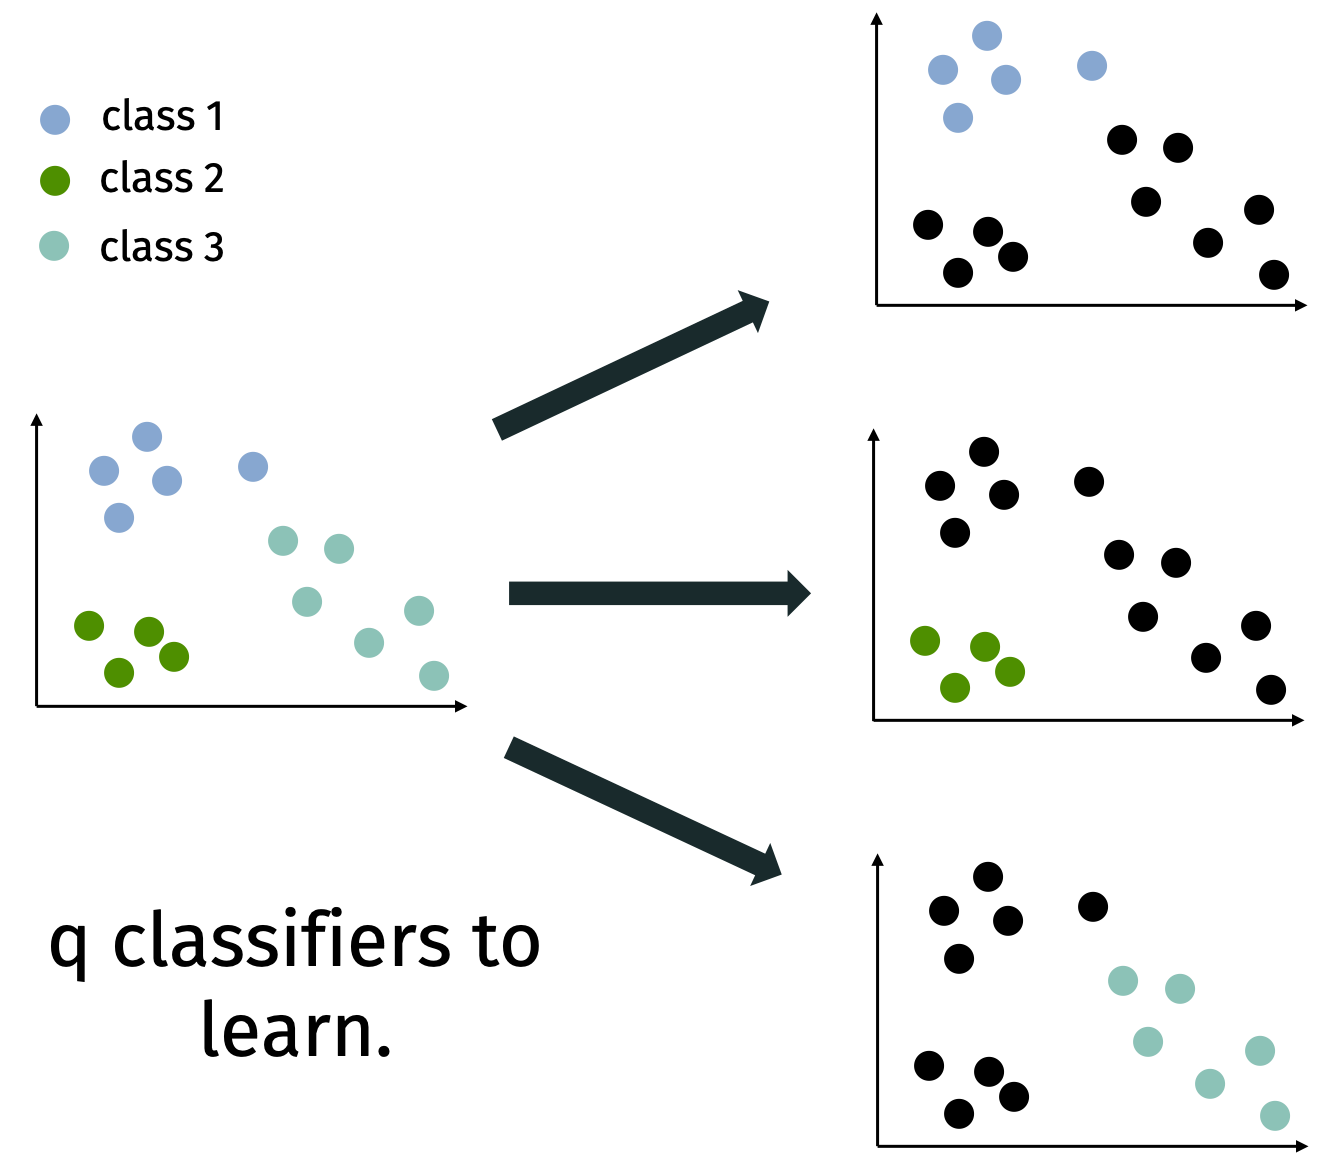
\includegraphics[width=.6\textwidth]{one_vs_all.png}
	\end{center}
	\vspace{-1em}
	\begin{itemize}
		\item For $q$ classes train $q$ classifiers. Obtain parameters $\vec{\beta}_1, \ldots, \vec{\beta}_q$.
		\item Assign $y$ to class $i$ with maximum $\langle\vec{\beta}_i,\vec{x}\rangle$.
	\end{itemize}
\end{frame}

\begin{frame}
	\frametitle{one vs. rest}
	\small
	\begin{center}
		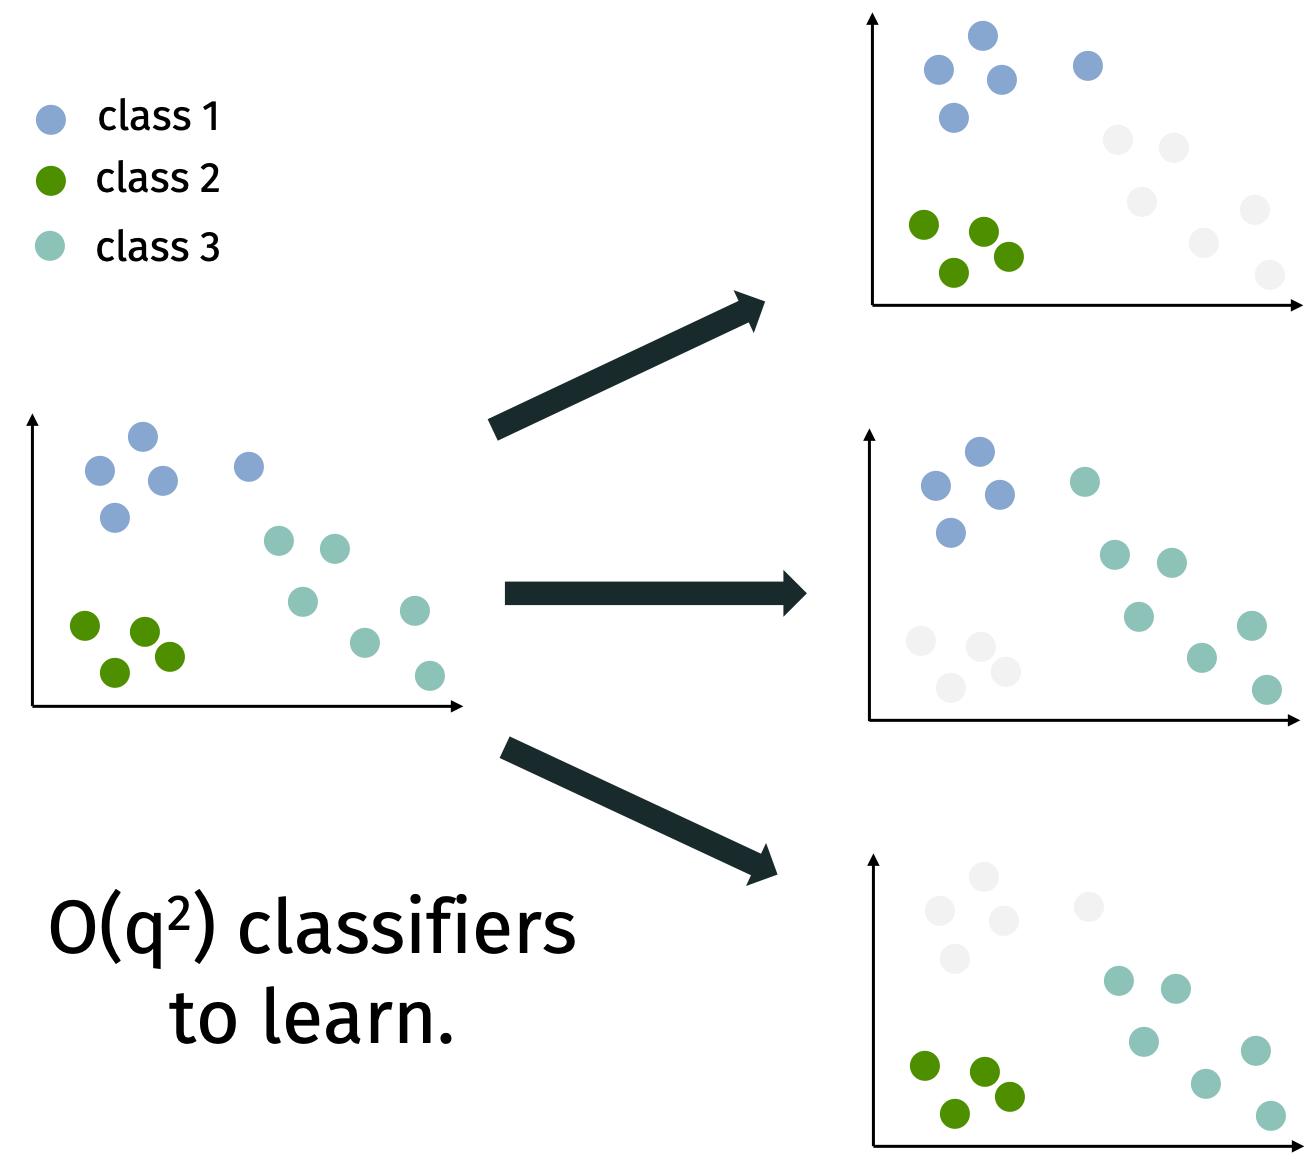
\includegraphics[width=.6\textwidth]{one_vs_one.png}
	\end{center}
	\vspace{-1em}
	\begin{itemize}
		\item For $q$ classes train $\frac{q(q-1)}{2}$ classifiers. 
		\item Assign $y$ to class which $i$ which wins in the most number of head-to-head comparisons. 
	\end{itemize}
\end{frame}

\begin{frame}
	\frametitle{one vs. one}
	\textbf{Hard case for one-vs.-all}.
	\begin{center}
		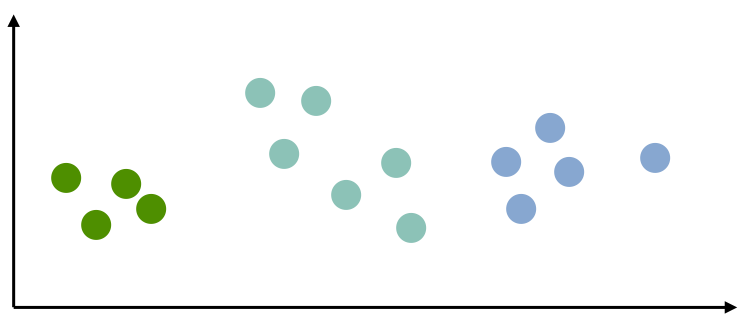
\includegraphics[width=.5\textwidth]{one_vs_hard.png}
	\end{center}
	\begin{itemize}
		\item One-vs.-one would be a better choice here. 
		\item Also tends to work better when there is class in balance.
	\end{itemize}
\end{frame}

\begin{frame}
	\frametitle{error in (multiclass) classification}
	\textbf{Confusion matrix} for $k$ classes:
	\begin{center}
		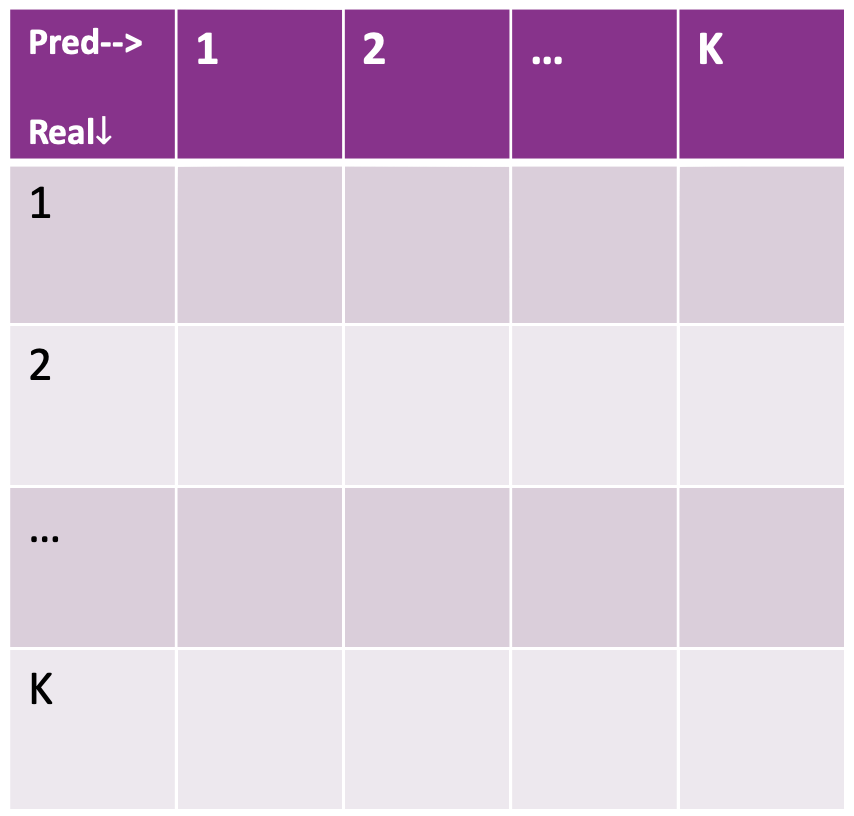
\includegraphics[width=.45\textwidth]{confusion_matrix.png}
	\end{center}
	\begin{itemize}
		\small
		\item Entry $i,j$ is the fraction of class $i$ items classified as class $j$.
		\item Overall accuracy is the \emph{average} of the diagonals.
		\item Useful to see whole matrix to visualize where errors occur.
	\end{itemize}
\end{frame}

\begin{frame}[t]
	\frametitle{logistic regression}
	Let $h_{\vec{\beta}}(\vec{x})$ be the \textbf{\alert{logistic function}}:
	\begin{align*}
	h_{\vec{\beta}}(\vec{x}) = \frac{1}{1 + e^{-\langle\vec{\beta},\vec{x}\rangle}}
	\end{align*}
	\begin{center}
		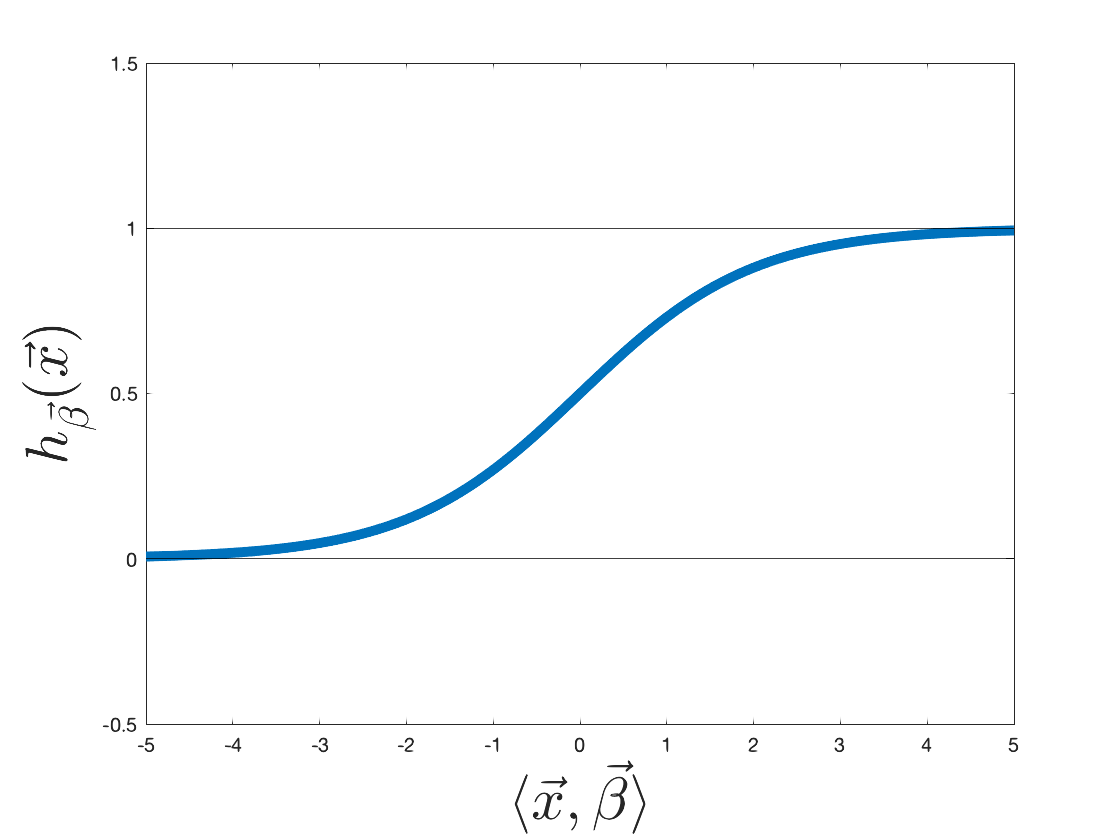
\includegraphics[width=.6\textwidth]{logistic_function.png}
	\end{center}
\end{frame}


\begin{frame}
	\frametitle{logistic regression}
	\begin{itemize}
		\item \textbf{Model}: Let $h_{\vec{\beta}}(\vec{x}) = \frac{1}{1 + e^{-\langle\vec{\beta},\vec{x}\rangle}}$
		\begin{align*}
		f_{\vec{\beta}}(\vec{x}) = \mathbbm{1}\left[h_{\vec{\beta}}(\vec{x})  > 1/2\right]
		\end{align*}
		\item \textbf{Loss function}: ``Logistic loss'' aka ``Cross-entropy loss''
		\begin{align*}
		L(\vec{\beta}) = - \sum_{i=1}^n y_i \log(h_{\vec{\beta}}(\vec{x})) + (1-y_i) \log(1 - h_{\vec{\beta}}(\vec{x})) 
		\end{align*}
	\end{itemize}
\begin{center}
	\large
	\alert{How do we find $\vec{\beta}$ which minimizes $L(\vec{\beta})$?}
\end{center}
\end{frame}

\begin{frame}
	\frametitle{logistic regression gradient}
	\vspace{-1em}
	\begin{align*}
	L(\vec{\beta}) = - \sum_{i=1}^n y_i \log(h_{\vec{\beta}}(\vec{x})) + (1-y_i) \log(1 - h_{\vec{\beta}}(\vec{x})) 
	\end{align*}
	Let $\bv{X}\in \R^{d\times n}$ be our data matrix with $\vec{x}_1, \ldots,\vec{x}_n \in \R^d$ as rows. Let $\vec{y} =[y_1, \ldots,  y_n]^T$. A calculation gives (see notes on webpage):
	\begin{align*}
		\alert{\nabla L(\vec{\beta})  = \bv{X}^T\left(h_{\vec{\beta}}(\bv{X}) - \vec{y}\right)}
	\end{align*}
	where $h_{\vec{\beta}}(\bv{X})  = \frac{1}{1+e^{-\bv{X}\vec{\beta}}}$. Here all operations are entrywise. I.e in Python you would compute:
	\vspace{-.5em}
	\begin{center}
		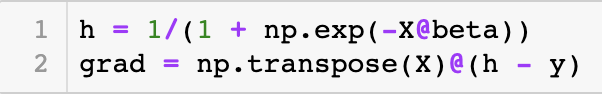
\includegraphics[width=.5\textwidth]{gradient_comp.png}
	\end{center}
\end{frame}

\begin{frame}
	\frametitle{logistic regression gradient}
	To find  $\vec{\beta}$ minimizing $L(\vec{\beta})$ we need to find a $\vec{\beta}$ where:
	\begin{align*}
	\nabla L(\vec{\beta})  = \bv{X}^T\left(h_{\vec{\beta}}(\bv{X}) - \vec{y}\right) = \vec{0}
	\end{align*}
	\begin{itemize}
		\item In contrast to what we saw when minimizing the squared loss for linear regression, there's no simple closed form expression for such a $\vec{\beta}$!
		\item This is \emph{the typical situation} when minimizing loss in machine learning: linear regression was a lucky exception.
		\item \textbf{Main question:} How do we minimize a loss function $L(\vec{\beta})$ when we can't explicitly compute where it's gradient is $\vec{0}$?
	\end{itemize}
\end{frame}

\begin{frame}[t]
	\frametitle{minimizing loss functions}
	\textbf{First idea.} Brute-force search. Test our many possible values for $\vec{\beta}$ and just see which gives the smallest value of $L(\vec{\beta})$. 
	\begin{itemize}
		\item As we saw on Lab 1, this actually works okay for low-dimensional problems (e.g. when $\vec{\beta}$ has 1 or 2 entries).
		\item \textbf{Problem:} Super computationally expensive in high-dimension. For $\vec{\beta} \in \R^d$, run time grows as:
	\end{itemize}
\end{frame}

\begin{frame}
	\frametitle{minimizing loss functions}
	\textbf{Much Better idea.} Some sort of \emph{\alert{guided}} search for a good of $\vec{\beta}$. 
\begin{itemize}
	\item Start with some $\vec{\beta}_0$, and at each step try to change $\vec{\beta}$ slightly to reduce $L(\vec{\beta})$. 
	\item Hopefully find an approximate minimizer for $L(\vec{\beta})$ much more quickly than brute-force search. 
	\item \textbf{Concrete goal:} Find $\vec{\beta}$ with $L(\vec{\beta}) < \min_{\vec{\beta}}L(\vec{\beta}) + \epsilon$ for some small error term $\epsilon$. 
\end{itemize}
\end{frame}

\begin{frame}
	\frametitle{gradient descent}
	\textbf{Gradient descent:} A greedy search algorithm for minimizing functions of multiple variables (including loss functions) that often works amazingly well.
	\begin{center}
		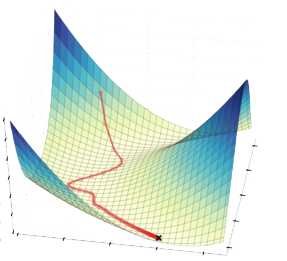
\includegraphics[width=.4\textwidth]{greedy_gradient.png}
	\end{center}
	\emph{The single most important computational tool in machine learning.} And it's remarkable simple + easy to implement.
\end{frame}

\begin{frame}
	\frametitle{optimization algorithms}
	
	\begin{center}
		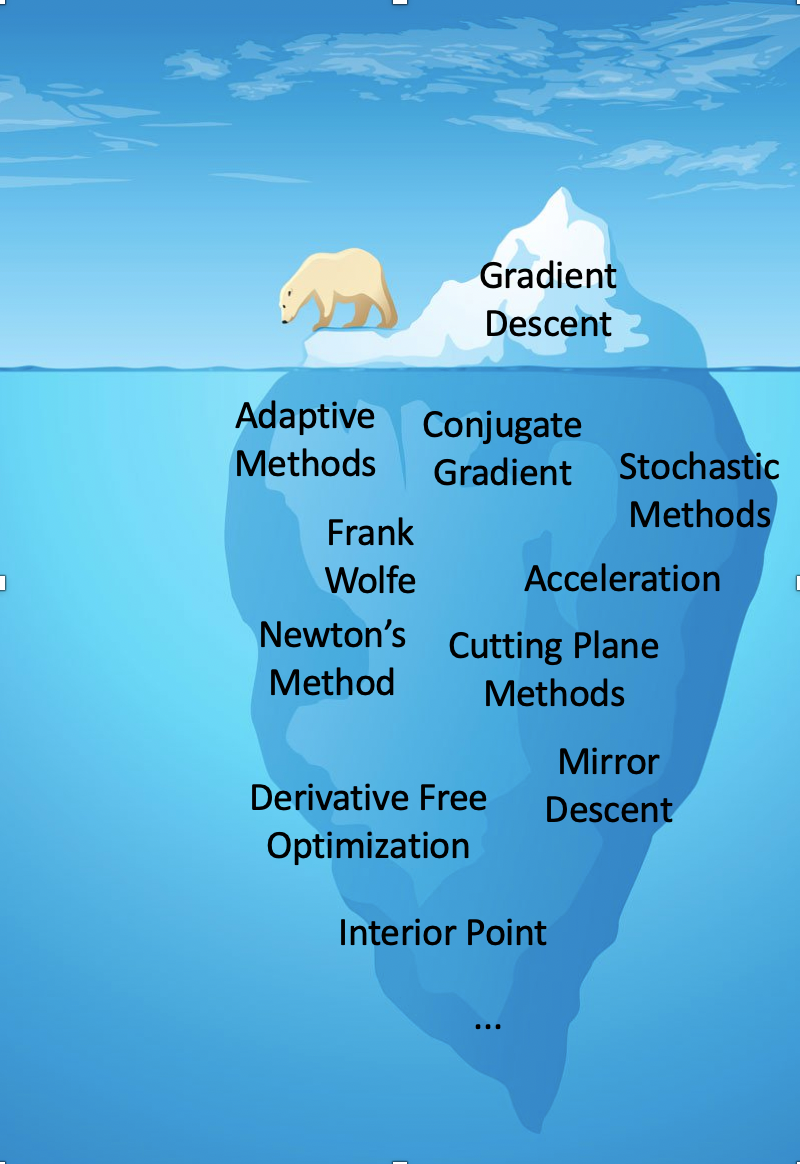
\includegraphics[height=.7\textheight]{iceberg.png}
		
		Just one method in a huge class of algorithms for \emph{numerical optimization}. All of these methods are important in ML: take my class in the fall (CS-GY 9223I) if you want to learn more. 
	\end{center}
\end{frame}


\begin{frame}
	\frametitle{first order optimization}
	\textbf{First order oracle model:} Given a function $L$ to minimize, assume we can:
	\begin{itemize}
		\item \textbf{Function oracle}: Evaluate $L(\vec{\beta})$ for any $\vec{\beta}$. 
		\item \textbf{Gradient oracle}: Evaluate $\nabla L(\vec{\beta})$ for any $\vec{\beta}$.
	\end{itemize}

	These are very general assumptions. Gradient descent will not use \emph{any other information} about the loss function $L$ when trying to find a $\vec{\beta}$ which minimizes $L$.
\end{frame}

\begin{frame}[t]
	\frametitle{intuition}
	Consider a $1$-dimensional loss function. I.e. where $\beta$ has just one entry:
	\begin{center}
		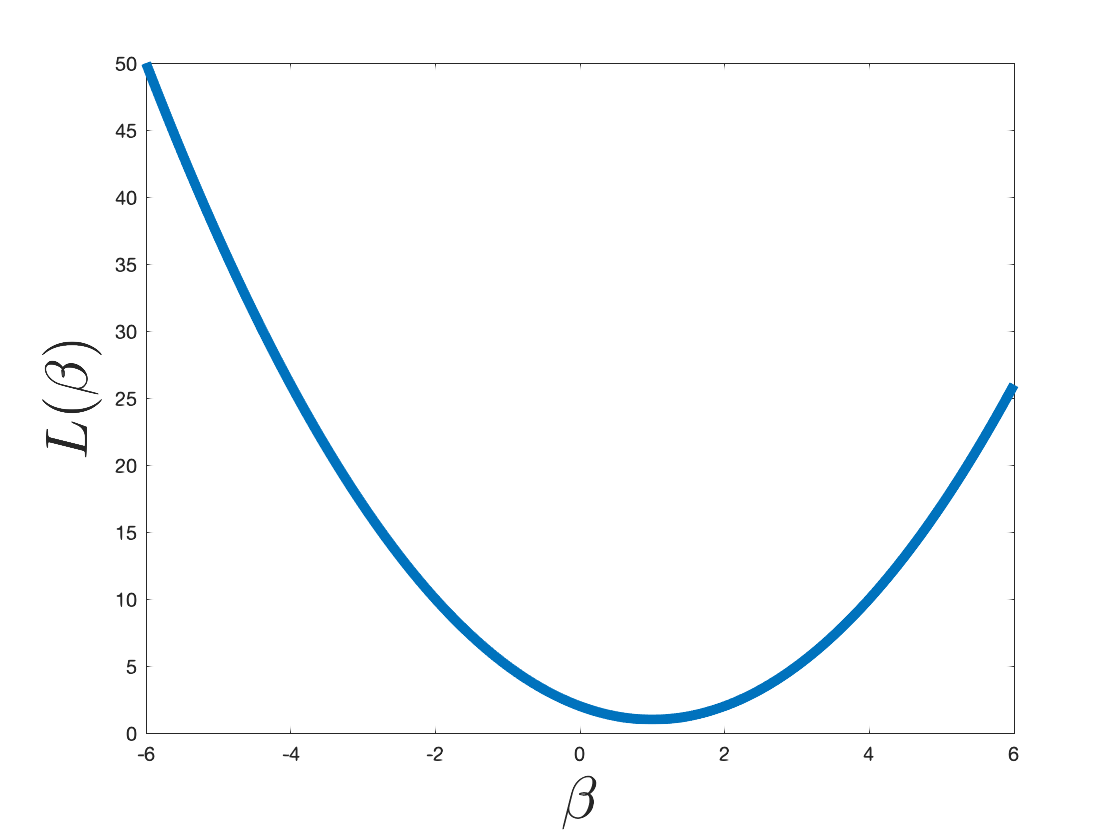
\includegraphics[width=.8\textwidth]{1d_example.png}
	\end{center}
\end{frame}

\begin{frame}[t]
	\frametitle{intuition}
	Consider a $1$-dimensional loss function. I.e. where $\beta$ has just one entry:
	\begin{center}
		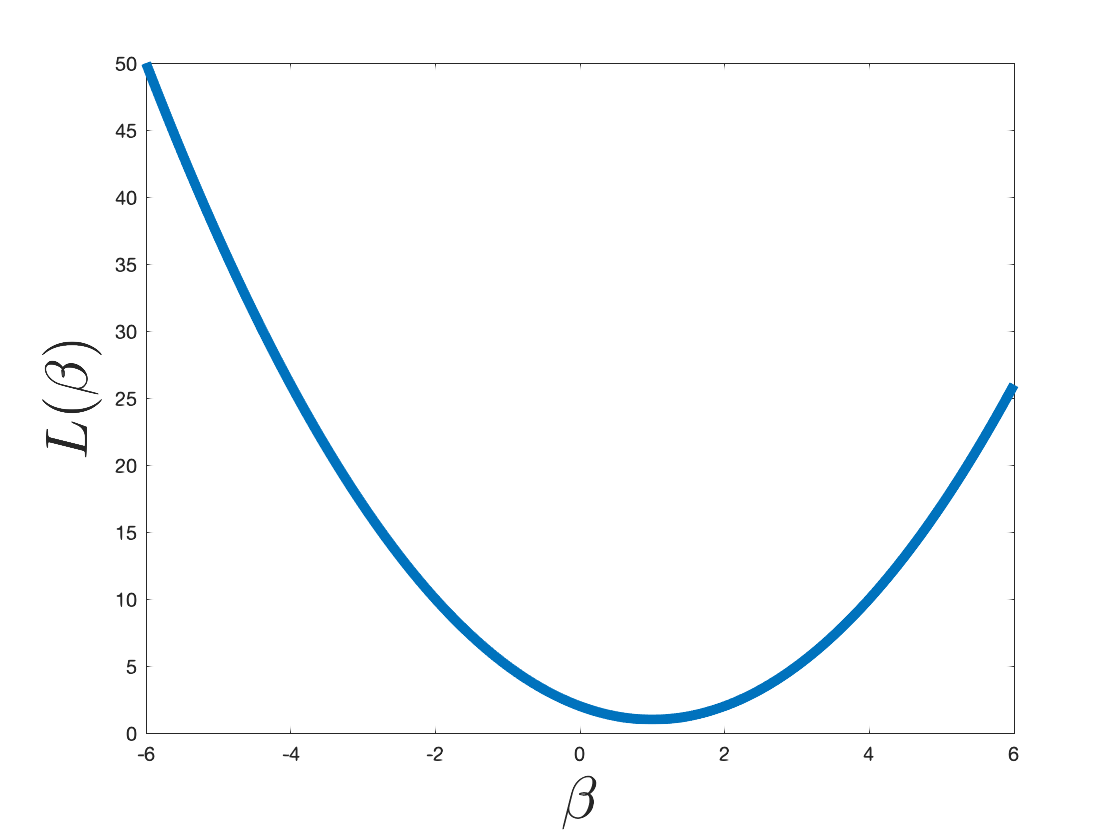
\includegraphics[width=.8\textwidth]{1d_example.png}
	\end{center}
\end{frame}

\begin{frame}
	\frametitle{gradient descent in 1d}
	\textbf{Recap:}
	\begin{itemize}
		\item Consider an algorithm which incrementally adjusts $\beta$. I.e. at each step $\beta \leftarrow \beta + \eta$ for some small $\eta$. Our goal is to ``make progress'' towards minimizing $L$, which means we want $L(\beta + \eta) < L(\beta)$. 
		\item For a 1D function, $\nabla L(\beta) = L'(\beta)$.
		\item So, for small $\eta$, $L(\beta + \eta) - L(\beta) \approx \nabla L(\beta)\cdot \eta$.
		\item Want right hand side $\nabla L(\beta)\cdot \eta$ to be \emph{negative}. 
		\item So choose $\eta$ to be positive if $\nabla L(\beta)$ is negative, and negative if $\nabla L(\beta)$ is positive.
	\end{itemize}

	\begin{center}
		\textbf{\alert{This is Gradient Descent (in 1D)!}}
	\end{center}
\end{frame}

\begin{frame}[t]
	\frametitle{directional derivatives}
	For high dimensional functions ($\vec{\beta}\in \R^d$), our update involves a vector $\vec{v} \in \R^d$. At each step:
	\begin{align*}
		\vec{\beta} \leftarrow \vec{\beta} + \vec{v}.
	\end{align*}
	
	\textbf{Question:} When $\vec{v}$ is small, what's an approximation for $L(\vec{\beta} + \vec{v}) - L(\vec{\beta})$?
	\begin{align*}
 		L(\vec{\beta} + \vec{v}) - L(\vec{\beta}) \approx \hspace{6em}
	\end{align*}
\end{frame}

\begin{frame}[t]
	\frametitle{directional derivatives}
	\begin{align*}
	L(\vec{\beta} + \vec{v}) - L(\vec{\beta}) &\approx \frac{\partial L}{\partial\beta_1} v_1 + \frac{\partial L}{\partial\beta_2} v_2 + \ldots + \frac{\partial L}{\partial \beta_d} v_d  \\
	& = \alert{\langle \nabla L(\vec{\beta}), \vec{v}\rangle.}
	\end{align*}
	
	\textbf{How should we choose $\vec{v}$ so that $L(\vec{\beta} + \vec{v}) < L(\vec{\beta})$?} 
\end{frame}

\begin{frame}[t]
	\frametitle{steepest descent}
	\begin{claim}[Gradient descent = Steepest descent\footnote{We could have restricted $\vec{v}$ using a different norm.  E.g. $\|\vec{v}\|_1 \leq 1$ or $\|\vec{v}\|_{\infty} \leq 1$. These choices lead to  variants of \emph{generalized steepest descent.}.}]
		$\frac{-\nabla L(\vec{\beta})}{\|\nabla L(\vec{\beta})\|_2} = \argmin_{\vec{v}, \|\vec{v}\|_2 \leq 1} \nabla \langle L(\vec{\beta}), \vec{v}\rangle$
	\end{claim}

\end{frame}

\begin{frame}[t]
	\frametitle{steepest descent}
	\begin{center}
		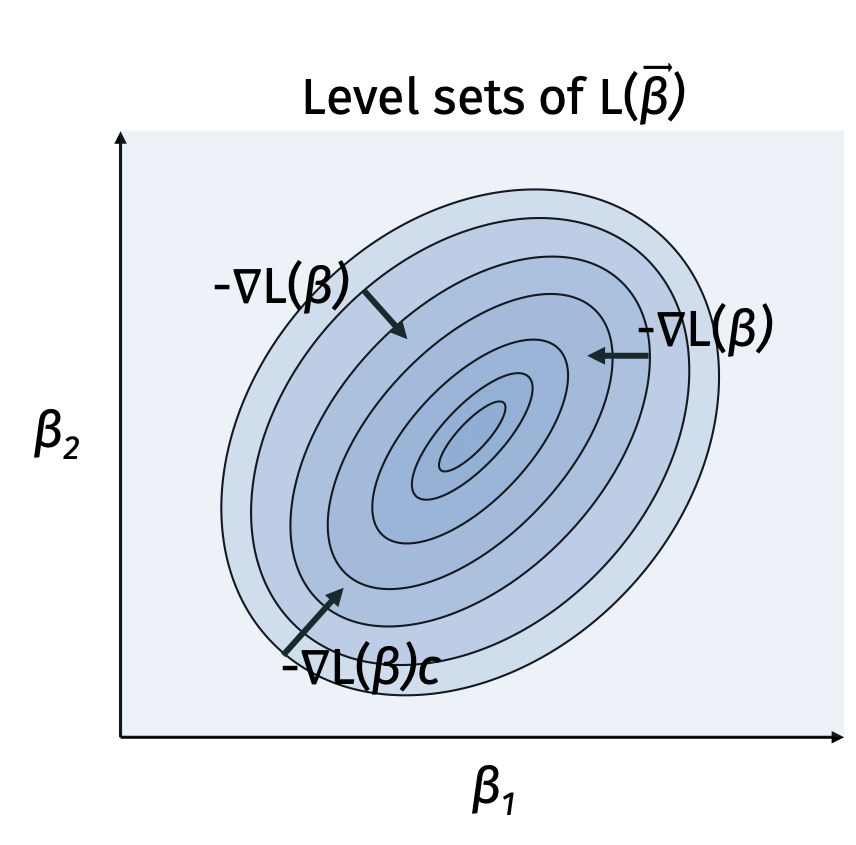
\includegraphics[width=.7\textwidth]{2d_example.png}
	\end{center}
\end{frame}

\begin{frame}
	\frametitle{gradient descent}
	\textbf{Gradient algorithm:}
	\begin{itemize}
		\item Choose arbitrary starting point $\vec{\beta}^{(0)}$.
		\item For $i = 1,\ldots, T$:
		\begin{itemize}
			\item $\vec{\beta}^{(i+1)} = \vec{\beta}^{(i)} - \eta \nabla L(\vec{\beta}^{(i)})$
		\end{itemize}
		\item Return $\vec{\beta}^{(t)}$.
	\end{itemize}
	
	$\eta$ is a \emph{step-size} parameter. Also called the \emph{learning rate}. Needs to be chosen sufficiently small for gradient descent to converge, but too small will slow down the algorithm. Often ``tuned'' by trying out many different values. 
\end{frame}

\begin{frame}[t]
	\frametitle{convergence of gradient descent}
	\begin{center}
		\textbf{Does gradient descent converge for all loss functions $L$?}
	\end{center}
\end{frame}

\begin{frame}[t]
	\frametitle{convergence of gradient descent}
	\begin{center}
		\textbf{In general GD only converges to a \alert{local minimum}.}
		
		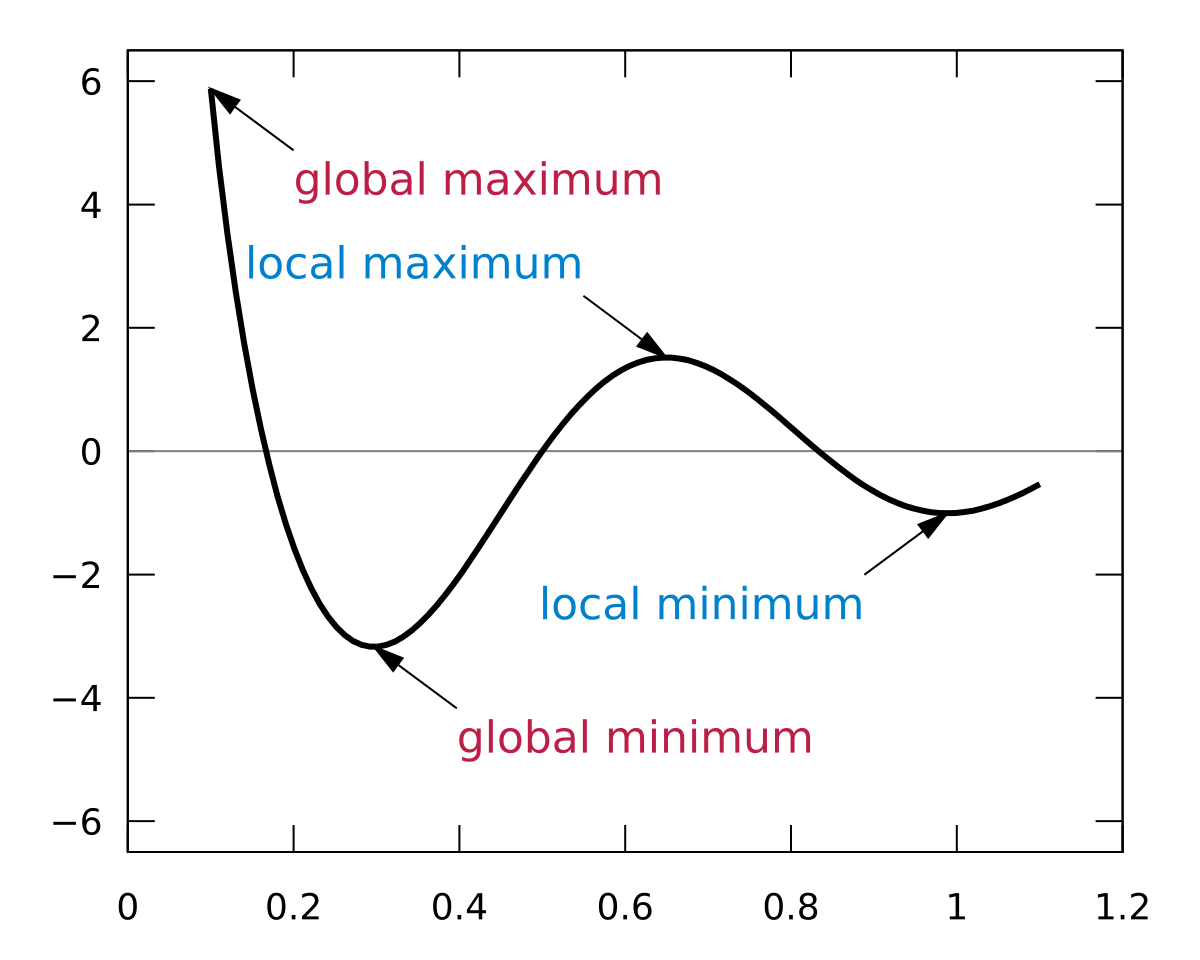
\includegraphics[width=.7\textwidth]{local_min.png}
	\end{center}
\end{frame}

\begin{frame}[t]
	\frametitle{convex function}
		\begin{definition}[Convex]
		A function $L$ is convex iff for any $\vec{\beta_1}, \vec{\beta_2},\lambda \in [0,1]$:
		\begin{align*}
		(1-\lambda)\cdot L(\vec{\beta_1}) + \lambda \cdot L(\vec{\beta_2}) \geq L\left((1-\lambda)\cdot\vec{\beta_1}+ \lambda \cdot\vec{\beta_2}\right)
		\end{align*}
		\vspace{-1em}
	\end{definition}
\vspace{-2em}
\begin{center}
	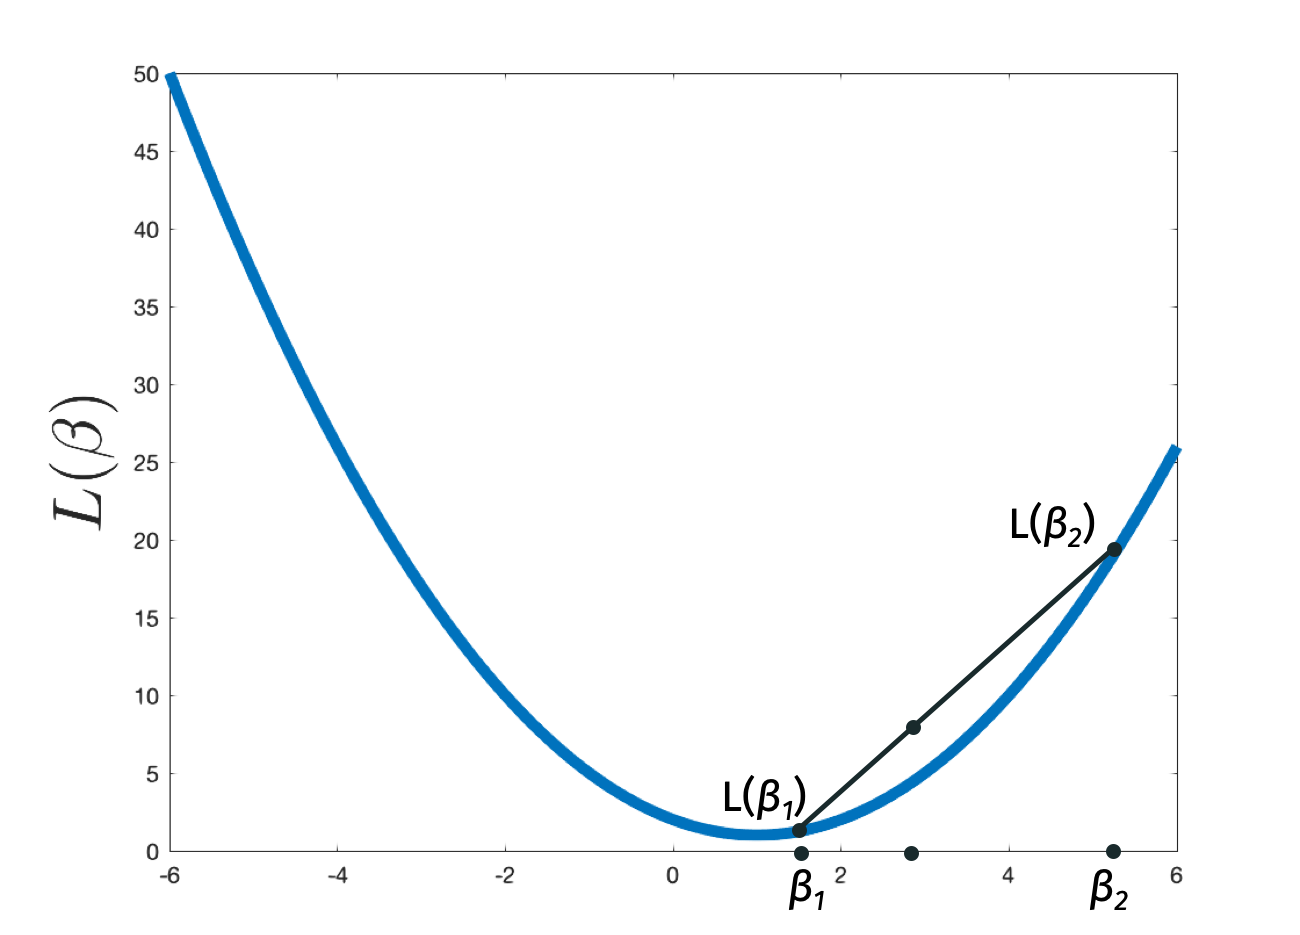
\includegraphics[width=.75\textwidth]{convex.png}
\end{center}
\end{frame}

\begin{frame}
		\frametitle{convex function}
	\textbf{In words:} A function is convex if a line between any two points on the function lies above the function. Captures the notion that a function looks like a bowl.
	
	\begin{center}
				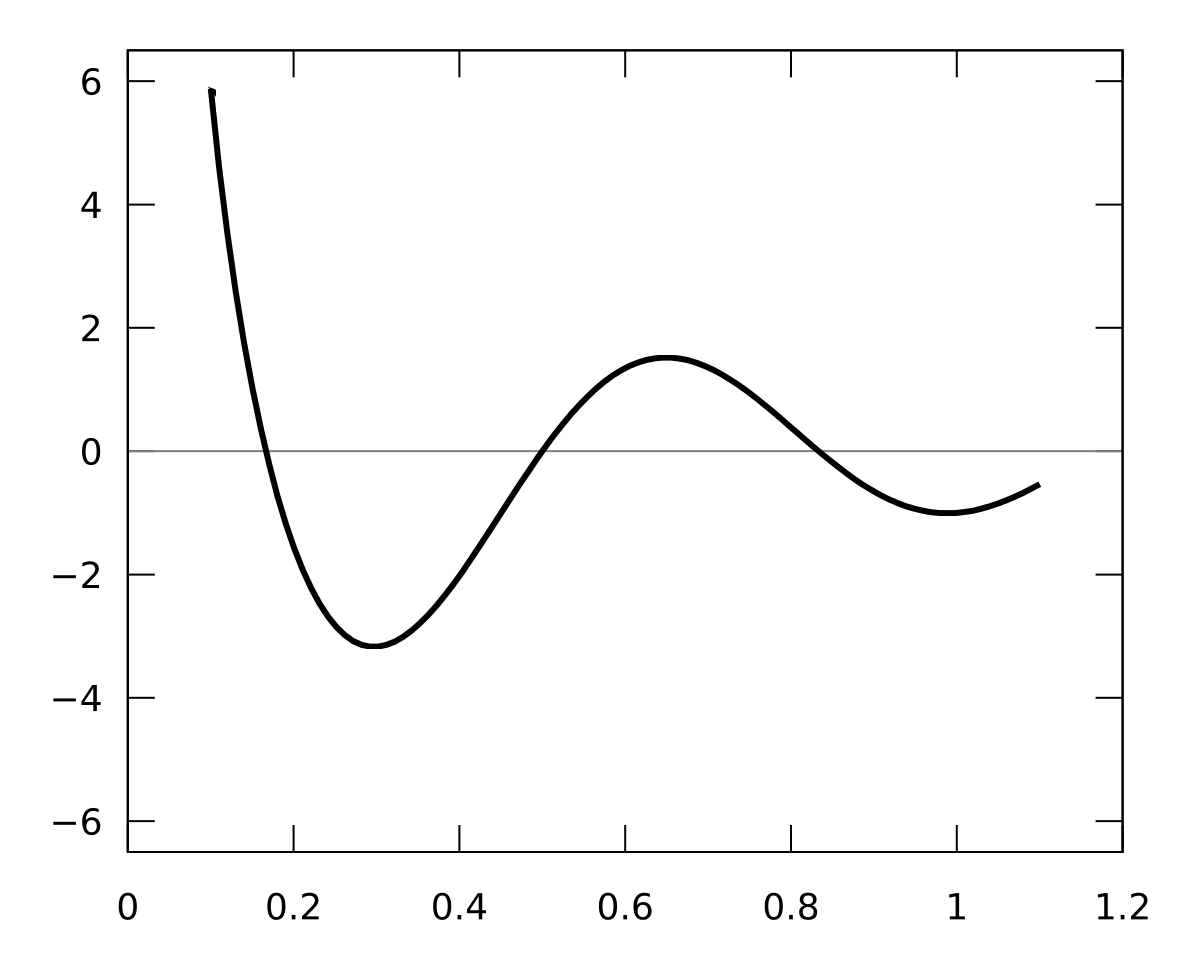
\includegraphics[width=.7\textwidth]{local_min_blank.png}
				
		This function is \textbf{not} convex.
	\end{center} 
	
\end{frame}

\begin{frame}[t]
	\frametitle{convex function}
		\begin{claim}[Convex Function Minimizers.]
		Every \emph{local} minimum of a convex function is also a \emph{global minimum}.
	\end{claim}
	
\end{frame}

\begin{frame}[t]
	\frametitle{convergence of gradient descent}
	\begin{claim}[GD Convergence for Convex Functions.]
		For sufficiently small step-size $\eta$, Gradient Descent converges to the global minimum of any convex function $L$.
	\end{claim}

	\textbf{What functions are convex?}
	\begin{itemize}
		\item Least squares loss for linear regression.
		\item $\ell_1$ loss for linear regression.
		\item Either of these with and $\ell_1$ or $\ell_2$ regularization penalty. 
		\item Logistic regression! Logistic regression with regularization.
		\item Many other models in machine leaning!
	\end{itemize}
\begin{center}
	This is not a coincidence: often it makes sense to reformulate your problem so that the loss function is convex, simply so you can minimize it with GD. 
\end{center}
\end{frame}

\begin{frame}
		\frametitle{convergence of gradient descent}
		Thing we will talk about after the midterm + spring break:
		\begin{itemize}
			\item Even though GD always converges for a convex function, it's \emph{rate of convergence} can vary widely. There are lots of methods to speed up the algorithm. 
			\item To implement GD, we need to compute $\nabla L(\vec{\beta})$ at every iteration. Typically pretty cheap, but not always for huge datasets. We will see an alternative approach called \emph{stochastic gradient descent} (SGD) to address this issue.
			\item What happens when we apply GD to \emph{non-convex} functions?  
		\end{itemize}
\end{frame}



\end{document} 






